\chapter{Hello World}
Vamos a escrita do primeiro programa em perl.  

\begin{figure}[!htb]
	\centering
	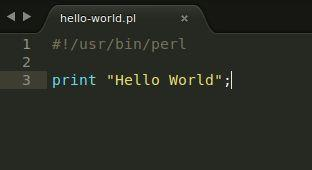
\includegraphics[width=0.3\textwidth]{../5_figuras/image1}
	\caption{Exemplo de implementa\c{c}\~ao}
\end{figure}

Na figura 1, a primeira linha ''\textit{\#!/usr/bin/perl}'', informa ao sistema que o c\'odigo passar\'a pelo interpretador perl, esta linha \'e 
necess\'aria para sistemas derivados do Unix, no Windows  o active perl configura uma instru\c{c}\~ao equivalente para o diret\'orio padr\~ao do sistema. 

Na 3$^a$ linha, o comando \textit{print} faz a escrita de dados para a sa\'ida padr\~ao de dados, neste caso, o monitor.  Sua sintaxe requer o uso de aspas duplas
por se tratar de um texto e o ponto e v\'irgula indica o fim de um comando.

Todo arquivo feito em Perl deve possuir a extens\~ao ''\textit{.pl}'', para executar um arquivo em Perl, deve-se abrir o promt ou o terminal e digitar o 
comando \textit{perl nomedoarquivo.pl} e pressionar Enter.
 